
\chapter{Platform description}
\section{Humanoid robot TEO}
Humanoid robot RH-2, also known as TEO (Task Environment Operator), from University Carlos III of Madrid, is and advanced version of humanoid robots RH-0 and RH-1. TEO is 165 cm high overtaking 150 cm of RH-1 and 120 cm of RH-0. It wheights about 60 kg and it can carry about 2 kg of payload. It has 24 DOFs (26 DOFs taking into account head motors), 3 more DOFs than in previous RH versions. In Figure \ref{ref:gdl} one can see the robot DOFs, besides their movements, being 6 DOFs for each leg, 6 DOFs for each arm, 2 DOFs for the torso and 2 DOFs for the head.

\begin{figure}[!hbt]
\centering
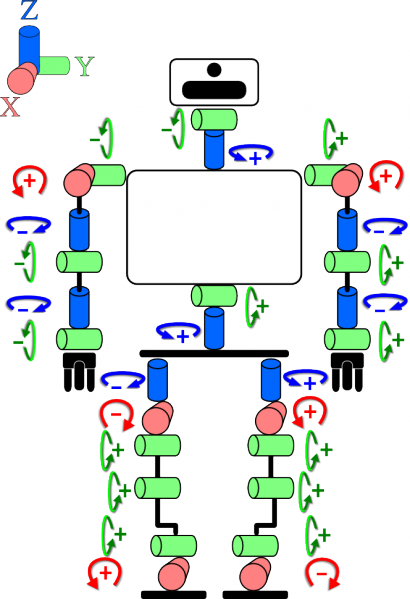
\includegraphics[scale=0.45]{teo_gdl.png}
\caption{Distribución de grados de libertad del robot TEO.}
\label{fig:gdl}
\end{figure}

The robot has 4 microprocessors: locomotion, manipulation, artificial vision tasks and last, the main processor which manages the others. The locomotion processor, that controls the legs and the torso, will be responsible for getting the sensors information and maintain the robot in a balance and upright position, being static or in a walking cycle. The manipulation processor controls the movement of the arms and the head. The processor responsible for the computer vision uses a camera with infrarred sensor ASUS located in the head.

The communication system is based on the CAN-bus protocol. Making a sagittal and transversal division, there are 4 CAN-bus lines: 1 line per each arm and neck, and 1 line per each leg and torso.

For data acquisition, the robot has Force-Torque sensors located at the robot ankles and wrists, used locomotion and manipulation, respectively. These sensors are plugged into real time data acquisition PCI cards. Including F/T sensors is an important difference and advantage respect RH-2 predecessors. They allow to close the control loop and then, to obtain a kind of feedback which is necessary to accomplish tasks successfully.


\section{Force/Torque sensors}
Force-Torque (F-T) sensors are based on strain gauge sensors arranged in such a way that allows to obtain force and moment measures in all axes of the 3D space. 

The sensors used in the platform, are the commercial JR3 F-T sensors described in Table\ref{table:sensores}. Look at the full scales difference between the sensors used in the wrists joints and the ones used in the ankle joints. Ankle sensors must be able to support greater forces and moments including the ones exerted by the own robot.

\begin{table}[!hbt]
\centering
\begin{tabular}{|c|c|c|c|c|}
\hline
Joint & Model & $F_{x,y}$ & $F_z$ & $M_{x,y,z}$\\
\hline
Wrist & 50M31A & 100N & 200N & 5 Nm\\ 
\hline
Ankle & 85M35A & 250N & 500N & 212Nm\\
\hline
\end{tabular}
\caption{F-T sensor models and characteristics. [JR3 Inc.]}
\label{table:sensores}
\end{table}

According to the manufacturer, the two first digits of the model show the sensor diameter, followed by the serie, and the next two digits, the thickness. As mentioned before, the ankle sensors are bigger and they support greater forces and moments. The sensors used in this Master Thesis are the ones mentioned in Table \ref{table:sensores} for ankle joints.

Serie M sensors include inner electronics in order to filter noise, digital output to use a data acquisition PCI card from the same manufacturer and an analogical output option. The nominal precission of all sensors of serie M is 1\% of full scale, and a 1/4000 full scale resolution.

\section{Data Acquisition}
The PCI cards used for data acquisition are PCI 1592D from JR3 Inc, which has 4 ports (named as in Figure ???). The sensors are plugged through a 6 or 8 pinouts (RJ-11 and RJ-45, respectively). In the case of RJ-45, two pinouts are not used. The PCI card uses these cables to receive high speed data and provide power supply to the sensors. About the PCI supply, it is provided by the PCI slot form the computer where it is installed.